\section{Numerical Experiments}

To implement and train the Triplet Network, we utilized PyTorch 2.0 \cite{Ansel_2024}, a framework designed for high-performance parallel computations on accelerated hardware. The Stochastic Quantization algorithm was implemented using the high-level API of Scikit-learn \cite{Pedregosa_2011}, ensuring compatibility with other package components (e.g., model training and evaluation), while leveraging NumPy \cite{harris2020array} for efficient tensor computations on CPU. All figures presented in this study were generated using Matplotlib \cite{Hunter_2007}. The source code and experimental results are publicly available in our GitHub repository \cite{Kozyriev_2024}.

For our experiments, we employed the original MNIST handwritten digit dataset \cite{lecun2010mnist} (see Fig.~\ref{mnist:fig}), comprising 60,000 grayscale images of handwritten digits with a resolution of 28x28 pixels, each associated with a class label from 0 to 9. Additionally, the dataset includes a corresponding set of 10,000 test images with their respective labels. It is noteworthy that we did not apply any data augmentation or preprocessing techniques to either the training or test datasets.

\begin{figure}
    \centering
    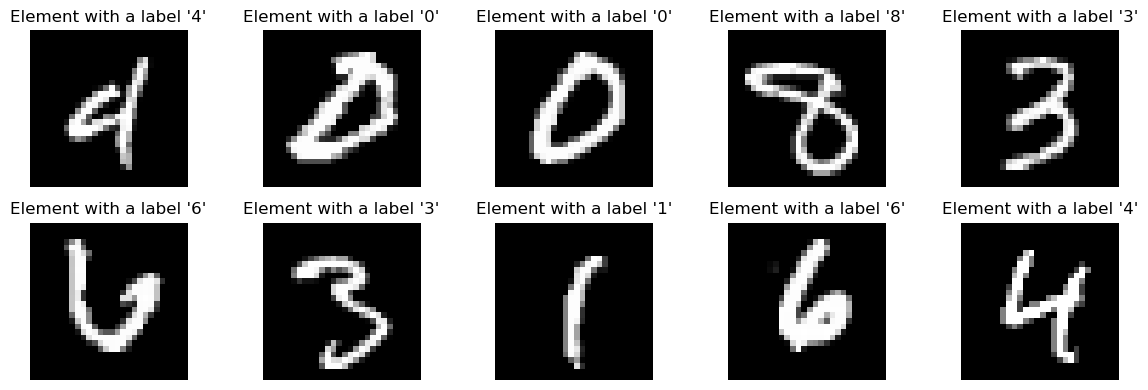
\includegraphics[width=\textwidth]{figures/dataset.png}
    \caption{Representative samples from the MNIST dataset \cite{lecun2010mnist} with their corresponding labels.}
    \label{mnist:fig}
\end{figure}

We approached the image classification task as a semi-supervised learning problem, training models on varying fractions of labeled training data (10\%, 30\%, 60\%, 80\%, and 100\%). The training dataset was split using uniform sampling into labeled and unlabeled portions according to the specified percentages. For the Triplet Network, we employed a Convolutional Neural Network architecture consisting of two Convolutional Layers with 3x3 filters (feature map dimensions of 32 and 64, respectively, with $\text{stride}=1$ and $\text{padding}=1$), followed by 2x2 Max-Pooling layers, and two Dense Layers. ReLU activation functions were used throughout the network. We trained separate Triplet Network models for each labeled data fraction with the following hyperparameters: 50 epochs, batch size of $1000 \times \text{fraction}$, learning rate $\rho = 10^{-3}$, and $l_2$ regularization rate $\lambda = 10^{-5}$. For the triplet loss (\ref{triplet-loss-func:eq}) and triplet mining (\ref{semi-hard-triplet-mining:eq}), we set the margin hyperparameter $\alpha = 1.0$. To facilitate meaningful feature capture while enabling visualization, we chose a latent space dimensionality of $\mathbb{R}^3$ (see Fig.~\ref{latent-space:fig}).

\begin{figure}
    \centering
    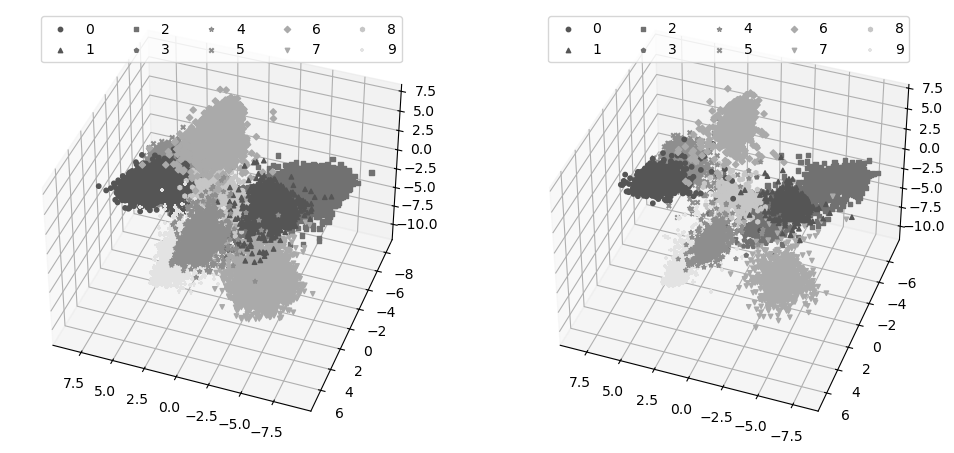
\includegraphics[width=0.9\textwidth]{figures/latent_space.png}
    \caption{Latent representations of images in the train dataset (left) and test dataset (right) projected by the Triplet Network, with each element color-coded according to its label (0-9). The clustering of elements with the same label suggests that the Triplet Network successfully captured relevant features during training.}
    \label{latent-space:fig}
\end{figure}

The Triplet Network was used to project latent representations onto $\mathbb{R}^3$ space from both labeled and unlabeled training data. These representations were then used to train the Stochastic Quantization algorithm as an unsupervised learning model. For each set of latent representations corresponding to different labeled data fractions, we trained the Stochastic Quantization algorithm and its adaptive variants (\ref{momentum-update-rule:eq}-\ref{adam-update-rule:eq}). We employed the K-Means++ initialization strategy (\ref{kmeans-plus-plus-init:eq}) for all variants, with a rank hyperparameter $r = 3$. To ensure convergence, we used different learning rates for each variant: $\rho = 0.001$ for SGD, Momentum, and NAG; $\rho = 0.9$ for AdaGrad; and $\rho = 0.01$ for RMSProp and ADAM. With these hyperparameters, all Stochastic Quantization variants converged to the global optima (see Fig.~\ref{quants:fig}), with most converging on the first iteration (see Fig.~\ref{convergence:fig}).

\begin{figure}
    \centering
    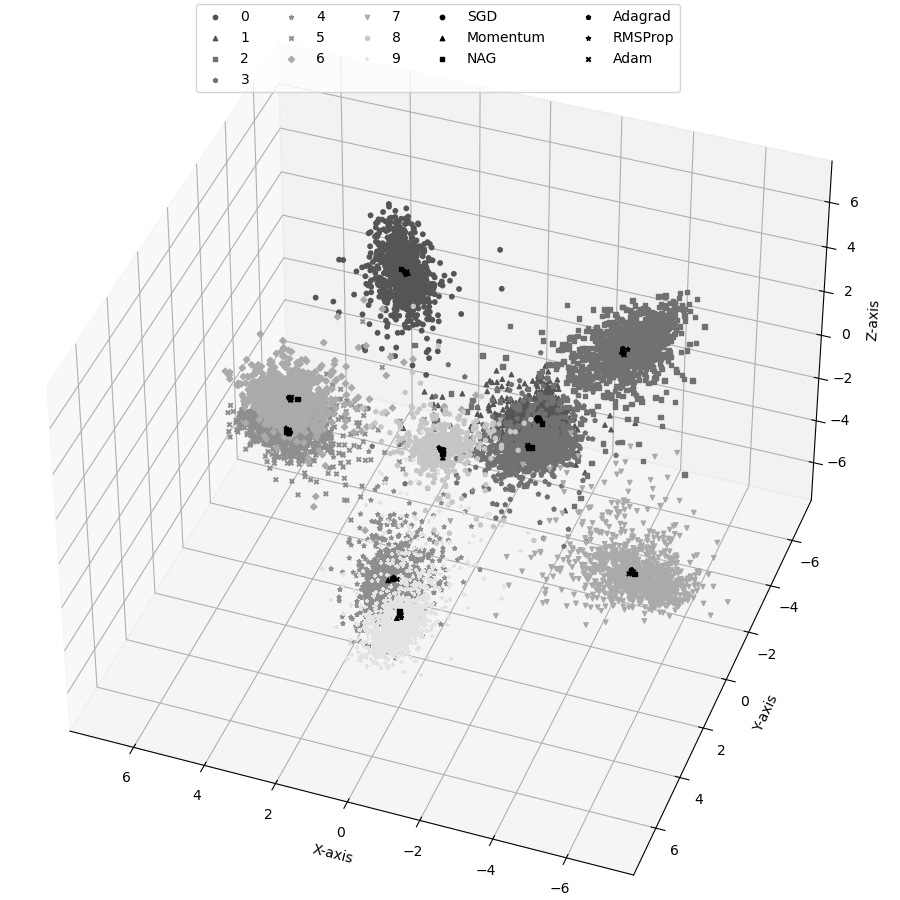
\includegraphics[width=0.9\textwidth]{figures/sq_quants.png}
    \caption{Optimal positions of quants for each Stochastic Quantization variant (labeled by variant name) in the latent space, relative to labeled elements (0-9) from the test dataset.}
    \label{quants:fig}
\end{figure}

\begin{figure}
    \centering
    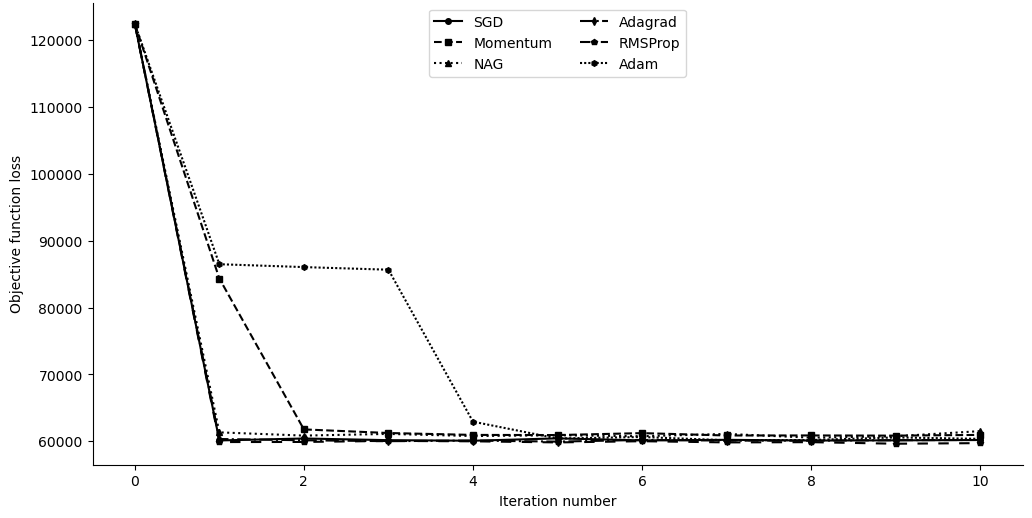
\includegraphics[width=\textwidth]{figures/sq_convergence_full_dataset.png}
    \caption{Convergence speed comparison of Stochastic Quantization variants on latent representations of training data with 100\% labeled fraction.}
    \label{convergence:fig}
\end{figure}

The accuracy of the trained classification models, combining Triplet Network and Stochastic Quantization, was evaluated using the F1-score metric \cite{Chinchor_1992} for weighted multi-label classification. Our experiments demonstrated that our approach achieved results comparable to state-of-the-art performance with Triplet Network and Siamese Network, as reported in \cite{Hoffer_2015}, even with limited labeled data:

\begin{table}
\caption{Classification accuracy comparison on MNIST dataset \cite{lecun2010mnist}.}
\label{accuracy:table}
    \begin{tabularx}{\textwidth}{|X|*{5}{c|}}
        \hline
        \multirow{2}{*}{Algorithm} & \multicolumn{5}{c|}{Percentage of Training Data} \\
        \cline{2-6}
        & 10\% & 30\% & 60\% & 80\% & 100\% \\
        \hline
        Triplet Network + KNN         & - & - & - & - & 99.54\% \\
        Siamese Network + KNN         & - & - & - & - & 97.90\% \\
        Triplet Network + SQ-SGD      & 94.67\% & 98.14\% & 98.23\% & 98.17\% & 98.26\% \\
        Triplet Network + SQ-Momentum & 92.97\% & 98.20\% & 98.26\% & 98.14\% & 98.24\% \\
        Triplet Network + SQ-NAG      & 94.12\% & 98.15\% & 98.29\% & 98.16\% & 98.25\% \\
        Triplet Network + SQ-AdaGrad  & 94.59\% & 98.11\% & 98.24\% & 98.18\% & 98.30\% \\
        Triplet Network + SQ-RMSProp  & 94.34\% & 98.16\% & 98.19\% & 98.17\% & 98.27\% \\
        Triplet Network + SQ-ADAM     & 93.01\% & 98.18\% & 98.23\% & 98.18\% & 98.25\% \\
        \hline
    \end{tabularx}
\end{table}